% %
% LAYOUT_E.TEX - Short description of REFMAN.CLS
%                                       99-03-20
% http://www.ctan.org/pkg/refman
%
% Updated for REFMAN.CLS (LaTeX2e)
%
\documentclass[a4paper]{refart}
\usepackage[utf8]{inputenc}
\usepackage[T1]{fontenc}
\usepackage[english]{babel}
\usepackage{lmodern}

\usepackage{makeidx}
\usepackage{acronym}
\usepackage[colorlinks=true]{hyperref}
\usepackage{tabularx}

% New page after each section
\usepackage{titlesec}
\newcommand{\sectionbreak}{\clearpage}

\usepackage[pdftex]{graphicx}
\graphicspath{{./figures/}}

\title{Communication Protocol Between Pedelec Station and Central Management System}
\author{
Authors:\\
RWTH - i5\\ \vspace{5mm}
Version:\\
0.0.1\\ \vspace{5mm}
Date:\\
\today}

\date{}
\emergencystretch1em  %

\pagestyle{myfootings}

\setcounter{tocdepth}{2}
\renewcommand{\arraystretch}{1.3}

\makeindex 

\begin{document}
\maketitle

\section*{Version History}

\begin{tabularx}{\linewidth}{ | l | l | X | }
  \hline
  \rowcolor{table-head}
  Version & Date & Description \\
  \hline
  0.0.1	& \date{01.07.2014} & Initial draft \\
  0.0.2	& \date{03.07.2014} & Added Update Firmware (by \acs{CMS}) and Firmware Status Notification (by \acs{PS}) \\
  		& 				   & Added Change \& Get Pedelec Configuration (by \acs{CMS}) \\
  0.0.3 & \date{08.07.2014} & Deleted maxBatteryRange from Charging Status Notification (by \acs{PS}) \\
  0.0.4 & \date{10.07.2014} & Added Upload Logs (by \acs{CMS}) and Logs Status Notification (by \acs{PS}) \\
  		& 				   & Added more parameters to Charging Status Notification (by \acs{CMS}) \\
  0.0.5 & \date{18.08.2014} & Updated station pedelec URLs in \autoref{cms:main} \\
  \hline
\end{tabularx}

\tableofcontents

\section*{Acronyms}

\begin{acronym}[Bash]
 \acro{PS}{Pedelec Station}
 \acro{CMS}{Central Management System}
\end{acronym}
\section{Introduction}

// TODO


\subsection{Use Cases}

\subsubsection{Station Boot}

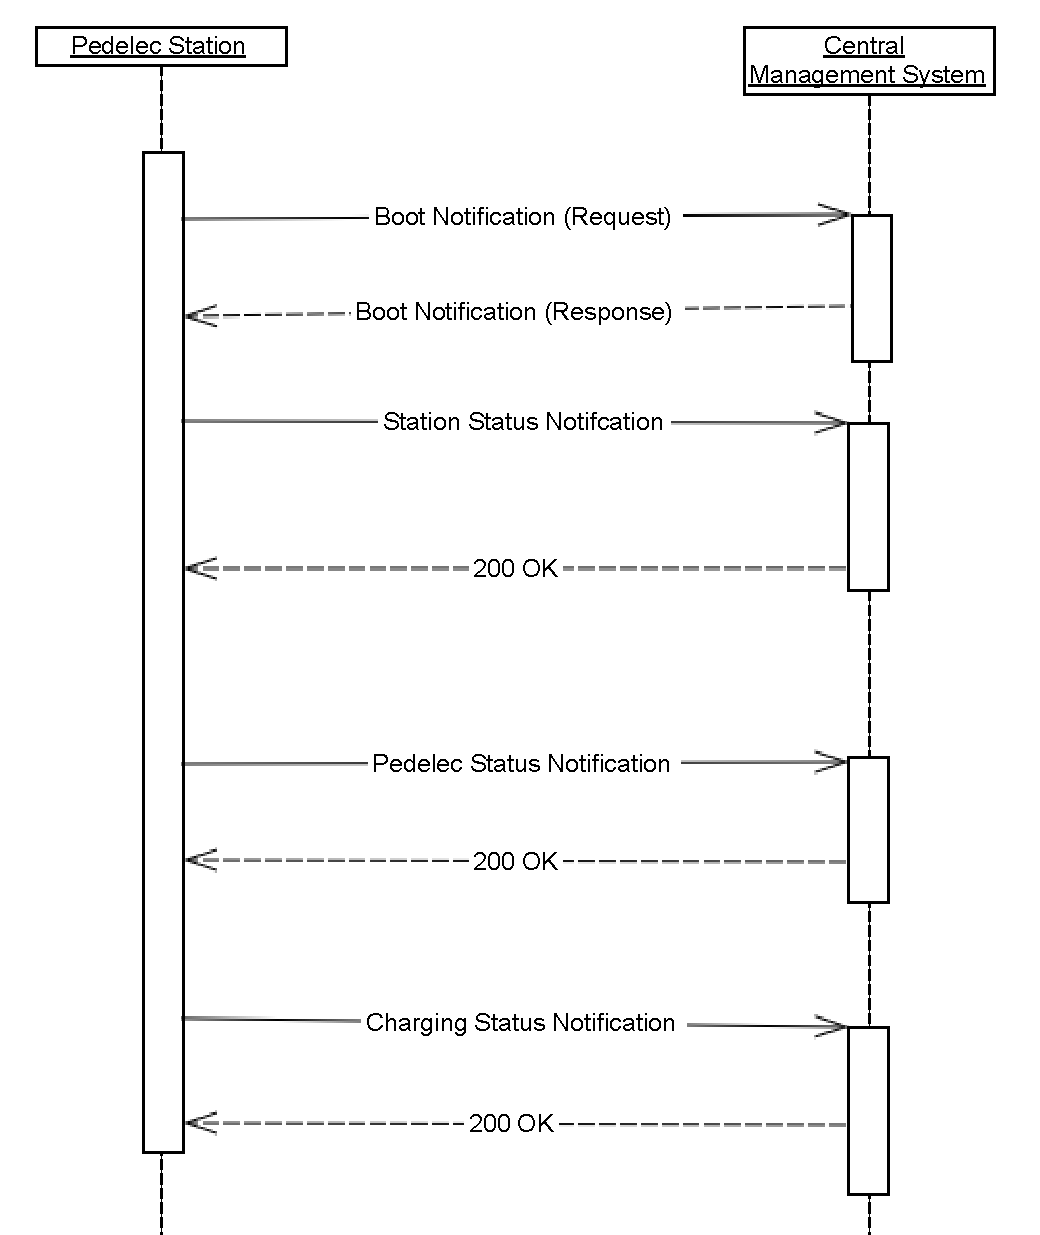
\includegraphics[scale=0.65]{station_boot_up.pdf}


\subsubsection{Rent Bike with Card}

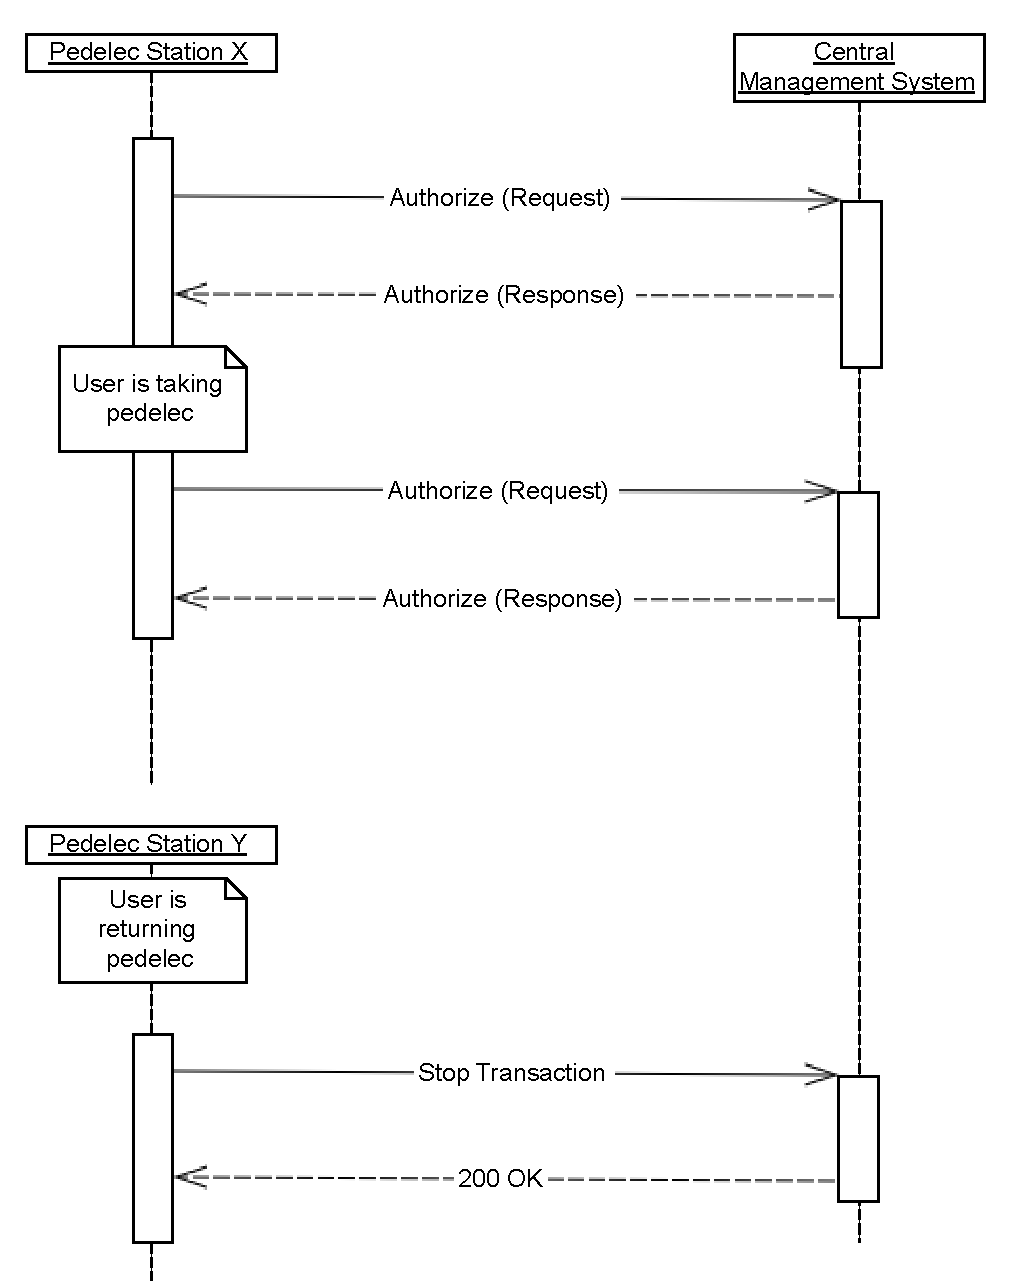
\includegraphics[scale=0.65]{rent_pedelec_with_card.pdf}

\subsubsection{Rent Bike with App}

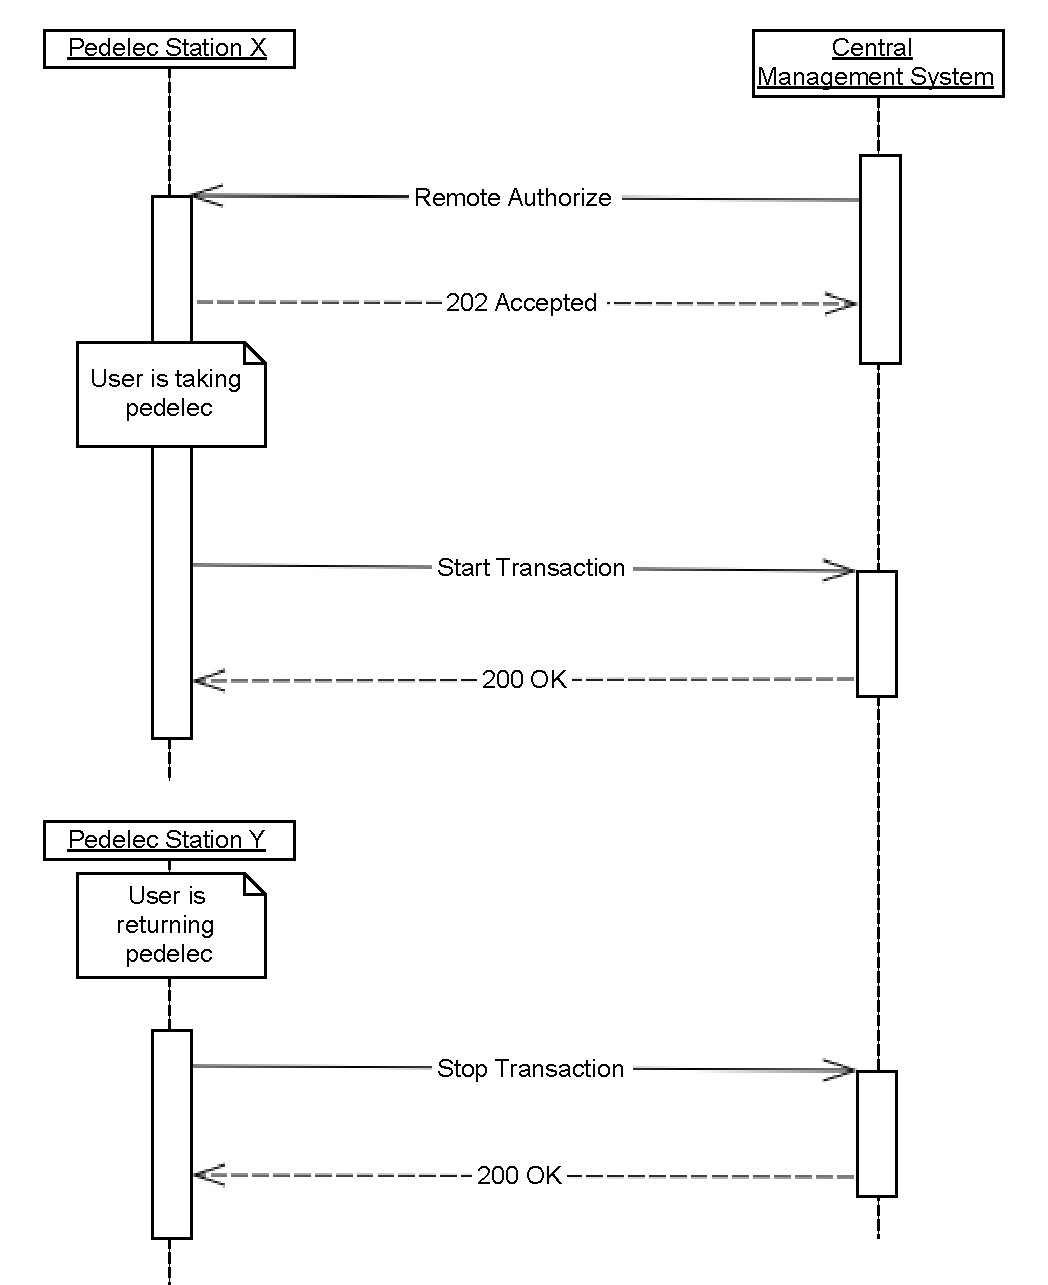
\includegraphics[scale=0.65]{rent_bike_with_app.pdf}


\subsection{Technology}

The protocol is designed to be implemented as a RESTful Webservice with HTTP as the underlying data transfer protocol. The resources are represented in JSON data format.

We require that all communications are done over SSL/TLS.
\section{Operations Initiated by PedelecStation}

\subsection{Boot Notification}

After start-up a Pedelec Station, the station sends a notification to the Central System with information about its configuration (e.g., manufacturer id, connected StationSlots and Pedelecs). Central System will accept only registered Stations. 

After each reboot, the Boot Notification is sent. 

The Central Systems responses if the Station is accepted, including current time and heartbeat interval if true.

The Stations repeats the Boot Notification (in an appropriated interval) until the Central System accepts the Station. The Station requests nothing else, until Central System accepts it.

\subsection{Station Status Notification}

A Station sends a notification to the Central System to inform the Central System about its status or error condition within the Station and the connected StationSlots. A Station shall send an StationStatusNotification when it becomes unavailable as a result of an error condition or other external events.

\subsection{Pedelec Status Notification}

A Station sends a notification to the Central System to inform the Central System about the status or error condition of connected Pedelecs. A Station shall send an PedelecStatusNotification when a Pedelec becomes unavailable as a result of an error condition or other external events.

\subsection{Authorize}

Before a user can choose and unlock a Pedelec (e.g, Bluecard), the Station needs to be able to authorize the operation. Only after authorization the Station will unlock the Pedelec. For this purpose the Station needs the Card-ID and PIN from the user for authorization.

The response shall indicate, whether or not the id, pin combination is accepted by the Central System.

\subsection{Start Transaction}

When a StationSlot unlocked a Pedelec and the Slot notifies the removal of the Pedelec by a user, the Station needs to inform the Central System about this.

The Central Station acknowledges.

\subsection{Stop Transaction}

After the Station recognizes the return of a Pedelec at a specific Slot, it needs to inform the Central Station about this.

\subsection{Heartbeat}

To let the Central Station know that a Station is still connected, a Station sends a heartbeat after a configurable time interval.

The Central Stations sends a response with the current time of the Central System, which could be used to synchronize the time of the Station with the time of the Central System.

\subsection{Charge State}
\section{Operations Initiated by CentralSystem}
\section{Types}

%\subsection{Standard API errors}
%\label{types:errors}
%
%\begin{tabularx}{\linewidth}{ | l | X | }
%  \hline
%  \textit{Code} & \textit{Description} \\
%  \hline \hline
%  400 		& Bad Request \\
%  401 		& Unauthorized \\
%  \hline
%\end{tabularx}

\subsection{Error Message Template}
\label{types:error-msg-template}

In case an error occurs, send an HTTP 400 (Bad Request) which \textit{always} responses with a JSON object containing following fields: 

\begin{tabularx}{\linewidth}{ | l | X | }
  \hline
  \rowcolor{table-head}
  Field & Description \\
  \hline
  timestamp & Unix timestamp (seconds since epoch)  \\
  code 		& Internal, application-specific error code \\
  message 	& Additional explanation \\
  \hline
\end{tabularx}


\marginlabel{Error Codes:}
\begin{itemize}
    \item AUTH\_ATTEMPTS\_EXCEEDED
    \item CONSTRAINT\_FAILED
    \item DATABASE\_OPERATION\_FAILED
    \item HARDWARE\_MALFUNCTION
    \item NOT\_REGISTERED
    \item PEDELEC\_MISSING
    \item PEDELEC\_FOUND
    \item UNKNOWN\_SERVER\_ERROR
\end{itemize}

\subsection{Operation State}
\label{types:OperationState}

\begin{tabularx}{\linewidth}{ | l | X | }
  \hline
  \rowcolor{table-head}
  Value & Description \\
  \hline
  OPERATIVE 		& When the item is functional and working and ready to serve \\
  INOPERATIVE 	& When the item is faulted and cannot be used \\
  \hline
\end{tabularx}

\subsection{Charging State}
\label{types:ChargingState}

\begin{tabularx}{\linewidth}{ | l | X | }
  \hline
  \rowcolor{table-head}
  Value & Description \\
  \hline
  CHARGING 		& When the battery is charging\\
  COMPLETED 		& When the charging process is completed \\
  NOT\_CHARGING 	& Neither charging nor completed\\
  \hline
\end{tabularx}

\subsection{Firmware Update State}
\label{types:FirmwareState}

\begin{tabularx}{\linewidth}{ | l | X | }
  \hline
  \rowcolor{table-head}
  Value & Description \\
  \hline
  DOWNLOAD\_FAILED & \acs{PS} failed to load firmware \\
  INSTALLATION\_FAILED & Installation of firmware failed \\
  INSTALLED & Firmware is successfully installed in \acs{PS} \\
  \hline
\end{tabularx}

\subsection{Logs Update State}
\label{types:LogUpdateState}

\begin{tabularx}{\linewidth}{ | l | X | }
  \hline
  \rowcolor{table-head}
  Value & Description \\
  \hline
  UPLOADED 		&  \\
  UPLOAD\_FAILED 	&  \\
  \hline
\end{tabularx}

% \subsection{Account State}
% \label{types:AccountState}

% \begin{tabularx}{\linewidth}{ | l | X | }
%   \hline
%   \rowcolor{table-head}
%   Value & Description \\
%   \hline
%   HAS\_PEDELEC 		& When customer occupies at least one pedelec \\
%   HAS\_NO\_PEDELEC 	& When customer has no pedelec  \\
%   \hline
% \end{tabularx}

\subsection{Configuration Error Reason}
\label{types:ConfigErrorReason}

\begin{tabularx}{\linewidth}{ | l | X | }
  \hline
  \rowcolor{table-head}
  Value & Description \\
  \hline
  NotAcceptable 		& If the request for some keys could not be processed. The server returns a JSON array of keys that are rejected (in this case other parameters are set) \\
  NotFound 	& If some of the keys are not found/supported. The server returns a JSON array of keys that are not found as configuration parameters (in this case other parameters are set) \\
  \hline
\end{tabularx}

%\subsection{Configuration Key-Value}
%\label{types:ConfigurationKeyValue}
%
%\begin{tabularx}{\linewidth}{ l l X }
%  \hline
%  \textit{Key} & \textit{Value} &\textit{Description} \\
%  \hline \hline
%  CentralSystemURL 	& string 	& New value for the URL \\
%\end{tabularx}

\end{document}


